\documentclass{beamer}
\usepackage[utf8]{inputenc}
\usetheme{default}
\usecolortheme{dove}
\usepackage{textpos}
\usepackage{grid-system}

% po4a: environment frame
% po4a: environment Row
% po4a: environment Cell


\title{Freifunk in Darmstadt}
\author{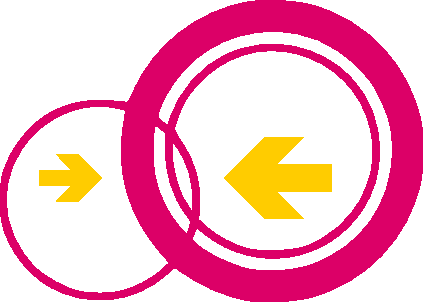
\includegraphics[width=4cm]{logo}}
%\institute[Inst.]{Freifunk Darmstadt}
\date{8. September 2014}

\begin{document}

\begin{frame}
\maketitle
\end{frame}

\addtobeamertemplate{frametitle}{}{%
\begin{textblock*}{100mm}(0.93\textwidth,-0.5cm)
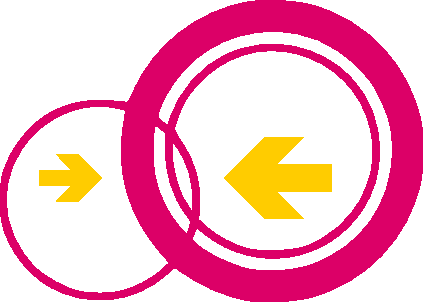
\includegraphics[height=1cm]{logo}
\end{textblock*}}

\begin{frame}{Outline}
\tableofcontents
\end{frame}

\section{Was ist Freifunk?}
\begin{frame}{Was ist Freifunk?}
\vfill
\begin{center}
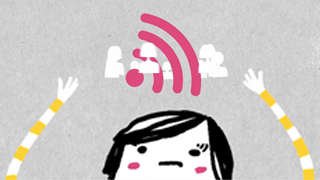
\includegraphics[width=0.5\textwidth]{up}
\end{center}
\vfill
Wie wäre es, wenn\ldots
\vfill
\begin{itemize}
\pause\item auch online jeder mit jedem kommunizieren könnte\pause , \textit{ohne eine Firma bei der man sich anmelden müsste?}
\vfill
\pause\item wir unsere eigenen Nachrichten, Filme, Musik, Radiostationen, Blogs, Bilderdienste und vieles mehr betreiben könnten\pause ,  \textit{ohne auf einen zentralen kommerziellen Anbieter angewiesen zu sein?}
\end{itemize}
\end{frame}

%\begin{frame}{Warum Freifunk?}
%\begin{center}\includegraphics[width=0.8\textwidth]{why}
%\vfill
%\pause We need private, free communication!

%Note for translation: private in terms of privacy, not ownership! :P )
%\end{center}
%\end{frame}


\begin{frame}{Wie sollte die Infrastruktur für unsere tägliche Kommunikation sein?}
\vfill
\begin{itemize}
\pause\item öffentlich
\pause\item anonym zugänglich
\pause\item nicht kommerziell
\pause\item unzensiert
\pause\item dezentral organisiert
\pause\item im Besitz einer Gemeinschaft
\end{itemize}
\vfill
\end{frame}


\section{Wie funktioniert Freifunk?}
\begin{frame}{Wie funktioniert Freifunk?}
\vfill
\centering
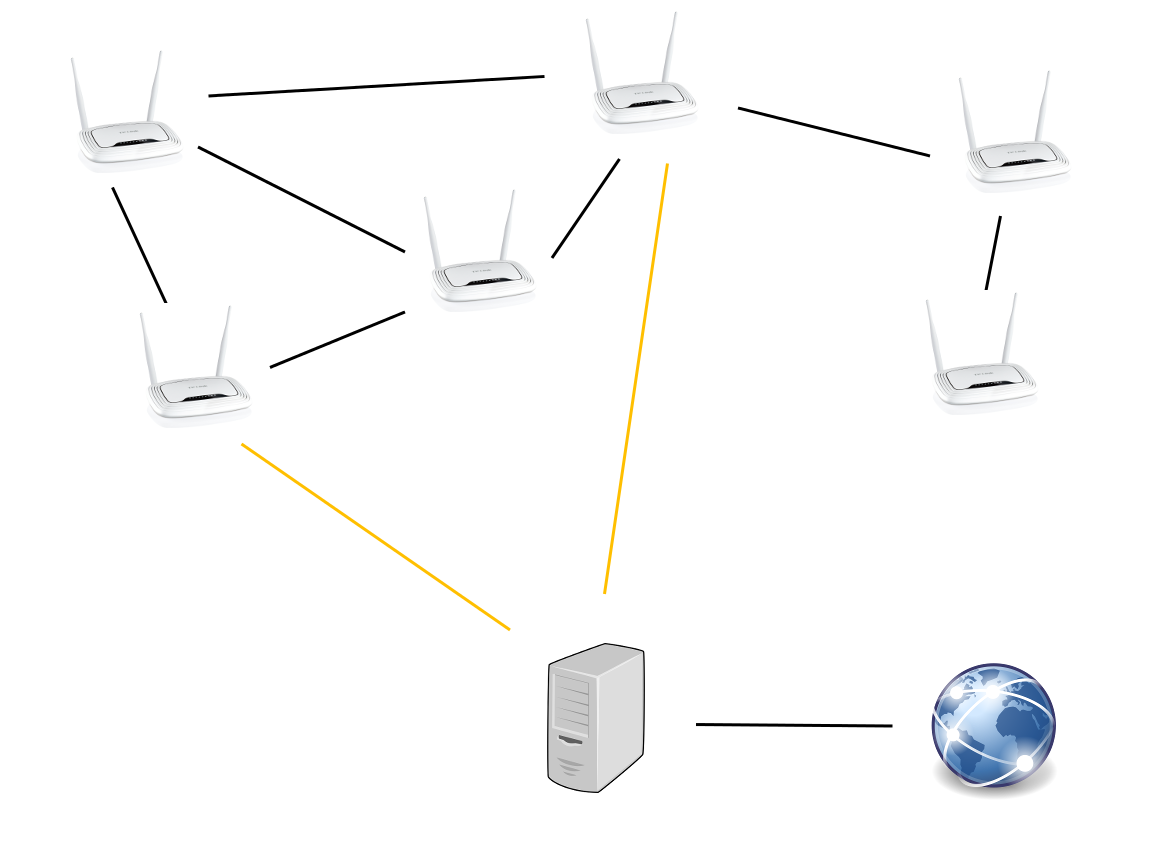
\includegraphics[height=6cm]{meshing}

Freifunk-Netze sind Netze aus WLAN-fähigen Geräten,\\ die sich untereinander verbinden,\\ ohne direkten Zugang zum Internet haben zu müssen.
\vfill
\end{frame}

\begin{frame}{Was kann man damit tun?}
\vfill
\begin{center}
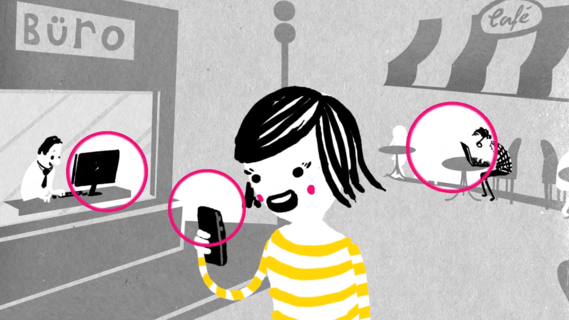
\includegraphics[width=5.5cm]{verbindet}
\end{center}

\begin{itemize}
\pause\item jeder kann Services anbieten und nutzen
%\pause\item z.B. mit kleinen, sparsamen Computern wie Raspberry Pi
\pause\item Telefonieren und Chatten
\pause\item dezentrales Social-Media (z.B Diaspora)
\pause\item lizenzfreies Community-Radio
\pause\item Austausch von Dateien und Medien (share+like)
\pause\item gemeinsame Nutzung eines Internetanschlusses
\pause\item Testbed f\"ur wissenschaftliche Experimente, \ldots
\end{itemize}
\vfill
\end{frame}

\section{Beispiele}
\begin{frame}{Wo gibt es schon Freifunk-Netze?}
\vfill
\centering
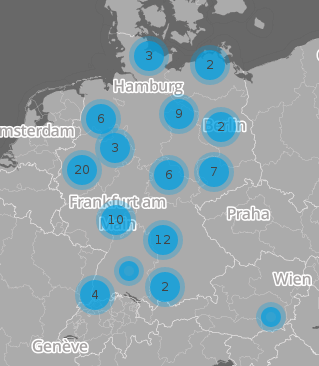
\includegraphics[scale=0.5]{map}
\vfill
über 100 lokale Gruppen, bundesweit knapp 4000 Accesspoints
\vfill
\end{frame}

\begin{frame}{Beispiel: Hamburg}
\vfill
\centering
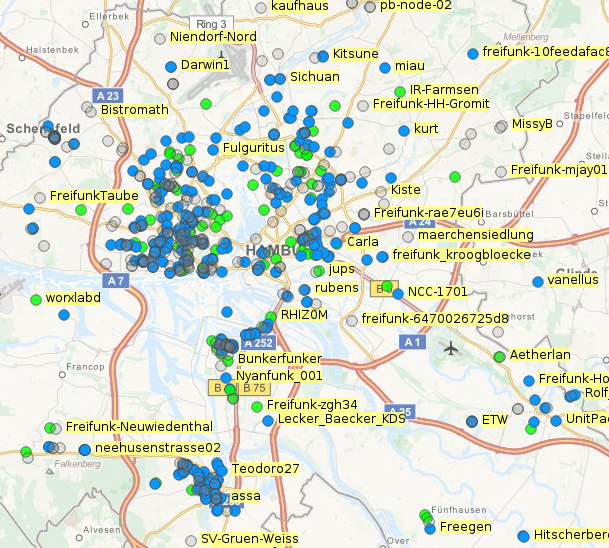
\includegraphics[scale=0.4]{hamburg-map}
\vfill
\end{frame}

\begin{frame}{Beispiel: Hamburg}
\vfill
\centering
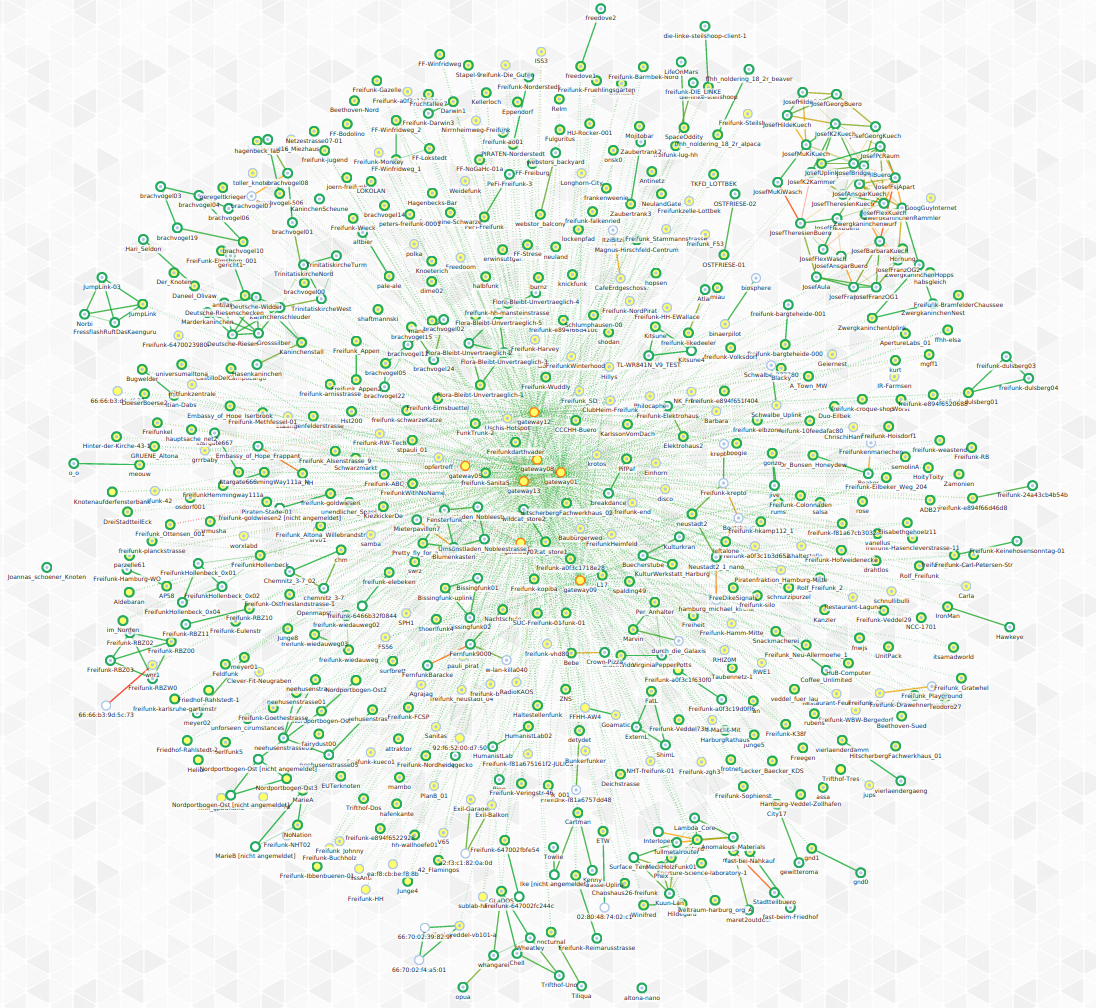
\includegraphics[scale=0.22]{hamburg-graph}
\vfill
\end{frame}

\begin{frame}{Beispiel: Mainz}
\vfill
\centering
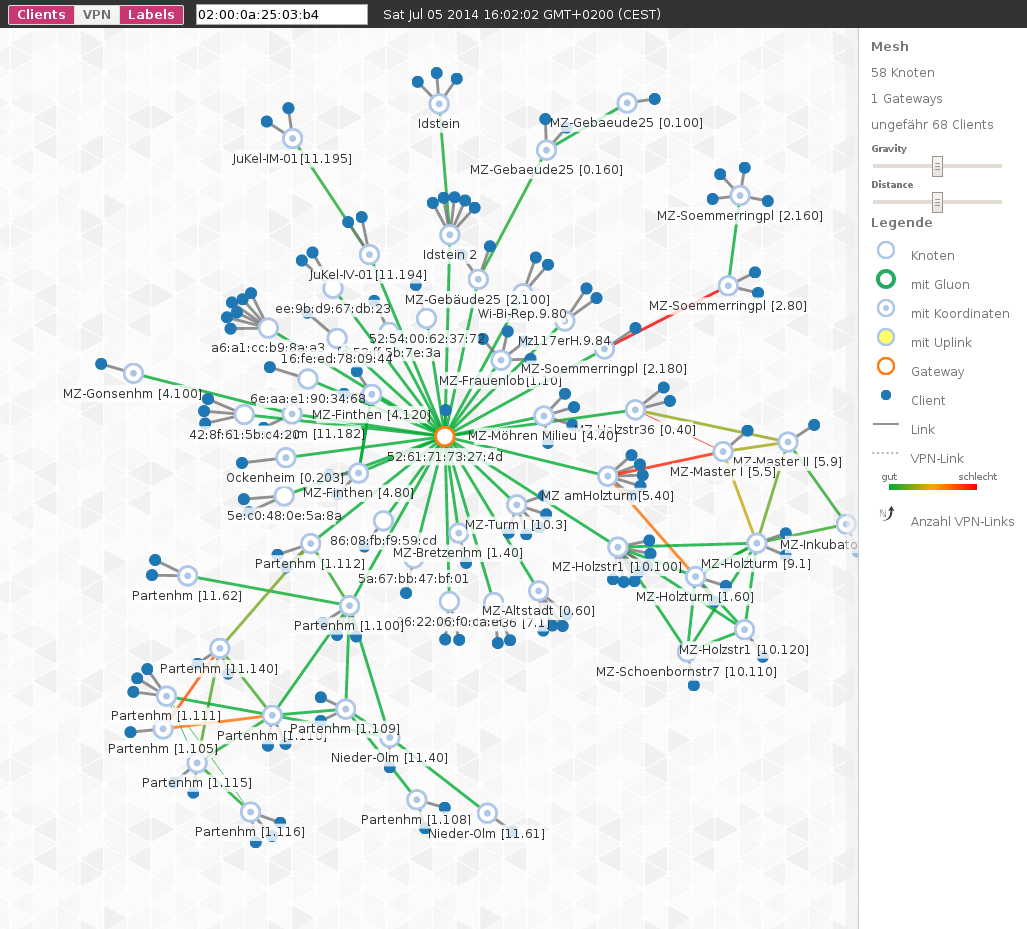
\includegraphics[scale=0.23]{mainz-nw}
\vfill
\end{frame}

\begin{frame}{Beispiel: Mainz}
\vfill
\centering
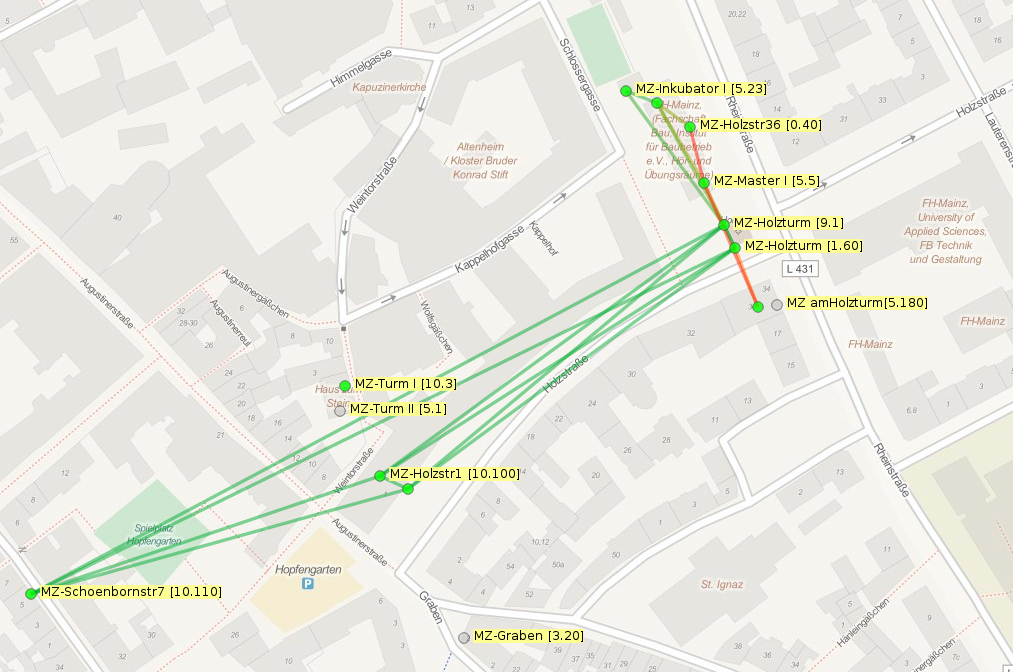
\includegraphics[width=\textwidth]{mainz}
\vfill
\end{frame}


\section{Was wollen wir für Darmstadt?}
\begin{frame}{Was wollen wir für Darmstadt?}
\begin{center}
\vfill
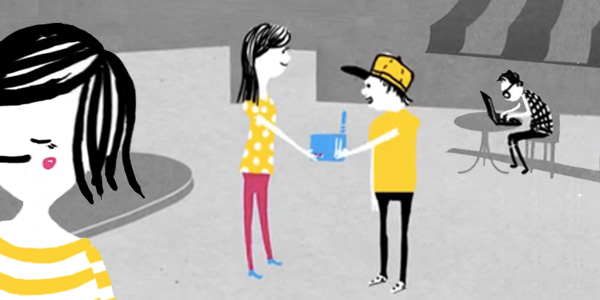
\includegraphics[width=0.6\textwidth]{router}
\end{center}

\vfill
Kurz und knapp: Unterstützer finden und viele Knoten verteilen!
\vfill
\end{frame}


\begin{frame}{Was wollen wir für Darmstadt?}
\vfill
Etwas ausführlicher\ldots
\begin{itemize}
\pause\item Netzwerk erweitern\pause, aber nicht nur \ldots
\pause\item Services anbieten
\pause\item Mit anderen Communities verbinden (ICVPN)
\pause\item Experimente mit unterschiedlichen Protokollen, Software und Hardware
\end{itemize}
\begin{center}
\vfill
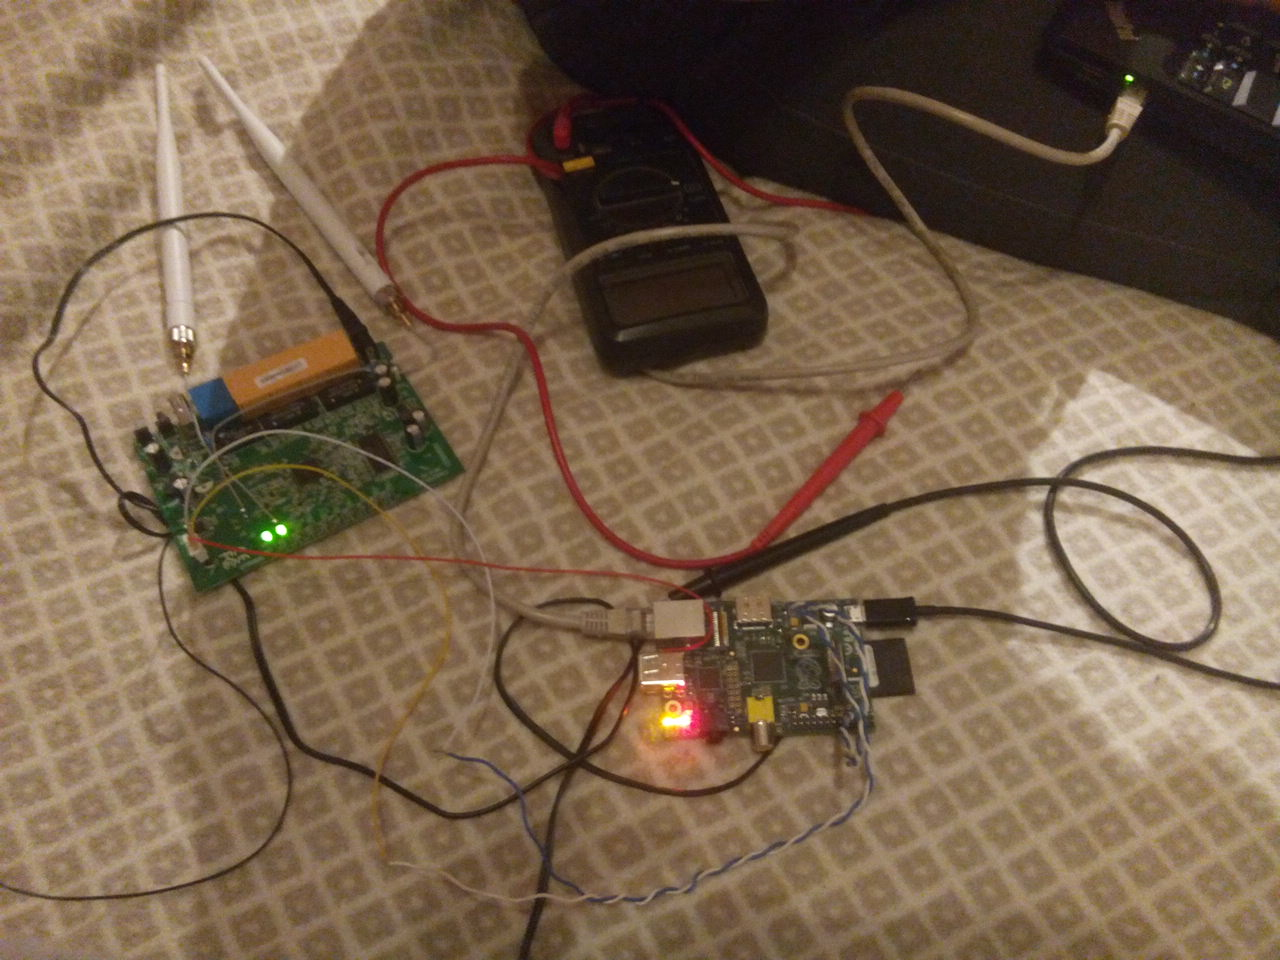
\includegraphics[width=0.4\textwidth]{disassemble}
\end{center}
\vfill
\end{frame}


\section{Aktueller Stand}
\begin{frame}{Aktueller Stand}
\vfill
\centering
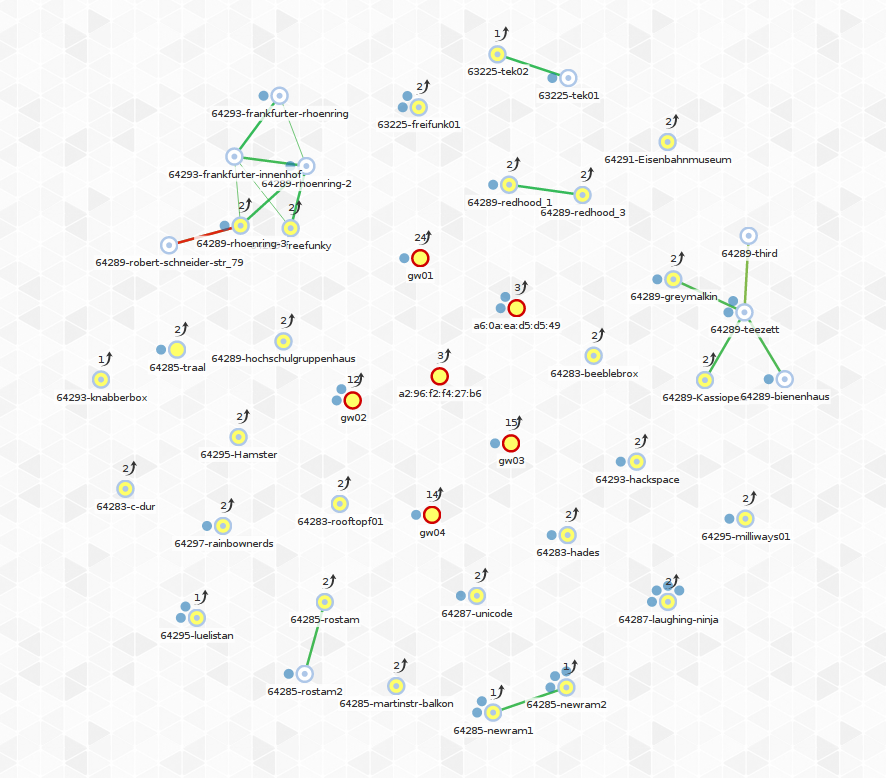
\includegraphics[scale=0.25]{darmstadt-graph}
\vfill
\end{frame}

\begin{frame}{Aktueller Stand}
\vfill
\centering
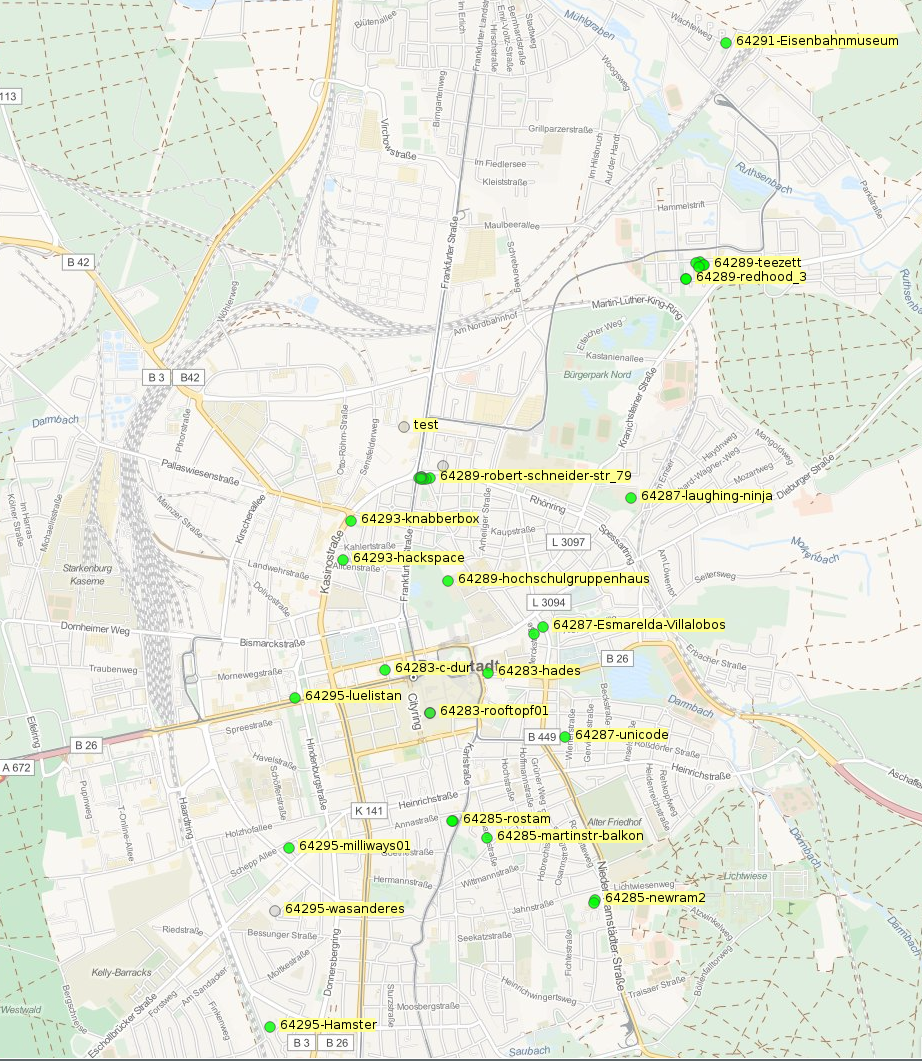
\includegraphics[scale=0.4]{darmstadt-map}
\vfill
\end{frame}


\section{Nächste Schritte}
\begin{frame}{Nächste Schritte}
\vfill
\begin{itemize}
\pause\item potentielle Unterstützer kontaktieren:
	\begin{itemize}
		\pause\item Einwohner
		\pause\item Geschäfte
		\pause\item Stadt
		\pause\item politische Gruppen
		\pause\item Unis
		\pause\item Studentenwohnheime, \ldots
	\end{itemize}
\pause\item Vorträge und Workshops organisieren
\pause\item Technik ausbauen und redundant machen
\pause\item Sponsoren finden für Technik und öffentliche APs
\end{itemize}
\vfill
\end{frame}

\section{Rechtliche Aspekte und Risiken}
\begin{frame}{Rechtliche Aspekte und Risiken}
\begin{Row}
\begin{Cell}{1}
\vspace{0.1cm}

\includegraphics[width=3.7cm]{recht}
\end{Cell}
\begin{Cell}{2}
\vspace{1cm}
Überblick:
\begin{itemize}
\pause \item Störerhaftung
\pause \item Risiken fürs eigene Netz
\pause \item Sicherheit im Freifunk-Netz
\pause \item was Freifunk (noch) nicht bietet
\end{itemize}
\end{Cell}
\end{Row}
\end{frame}

\begin{frame}{Störerhaftung}
\begin{itemize}
\pause\item Teilen des eigenen Internetanschlusses ist in Deutschland legal
\begin{itemize}
	\pause\item \textbf{aber:} Mithaftung für illegale Aktivitäten, wenn Täter nicht zu ermitteln ist
\end{itemize}
\pause\item Abmahnkosten sind zu tragen
\vfill
\pause\item aktuelle Lösung: VPN in Länder ohne Störerhaftung
\pause\item Zukunft: selbst Provider werden
\end{itemize}
\vfill
\centering
\pause \textbf{Fazit:}\\Störerhaftung existiert noch, wir machen es aber sehr schwer,\\den eigentlichen Anschlussinhaber zu finden.

\end{frame}

\begin{frame}{Risiken fürs eigene Netz}
\vfill
\begin{center}
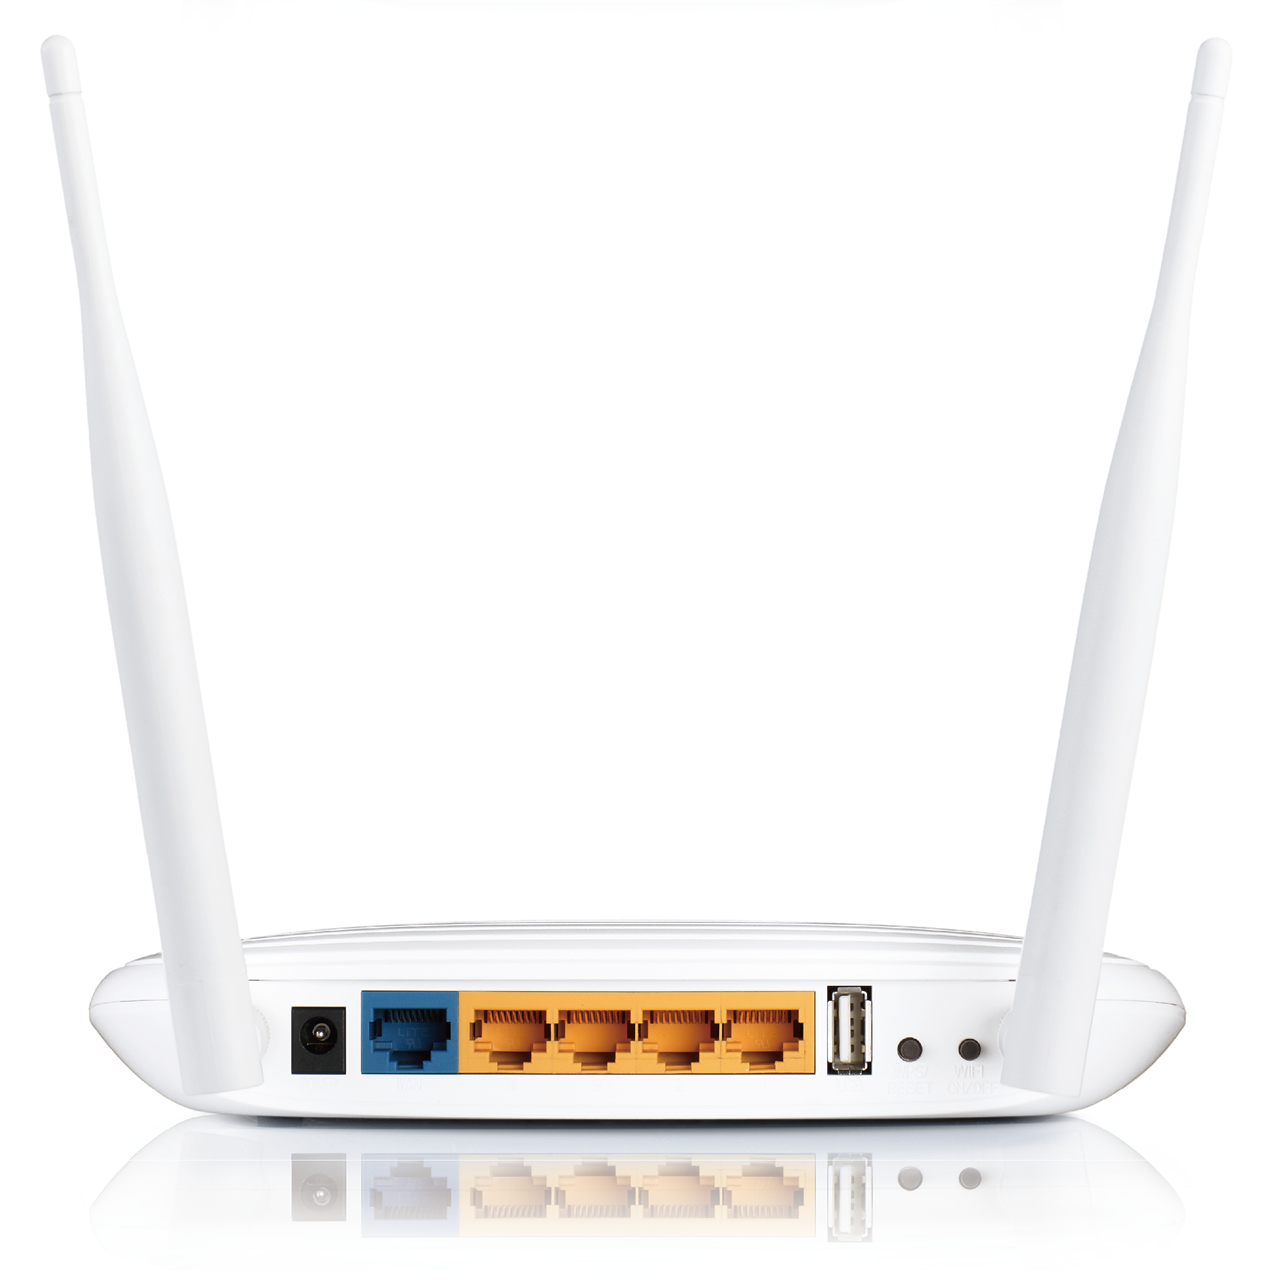
\includegraphics[height=4cm]{WR842ND-back}
\end{center}
\begin{itemize}
\pause\item Datenverkehr getrennt
\pause\item eigener Internetzugang nur für VPN zu anderen Knoten im Freifunk-Netz
\pause\item eigenes Netz und Freifunk-Netz sind getrennt, so lange Firmware keine Fehler hat oder gehackt wird
\end{itemize}
\vfill
\end{frame}

\begin{frame}{Sicherheit im Freifunk-Netz}
\begin{itemize}
	\pause\item Freifunk als freies Netz hat wenige Einschränkungen
	\pause\item Menschen können darin auch böse Dinge tun
	\vfill
	\pause\item Daten im Freifunk-Netz: Gesamter Verkehr schwer zu überwachen, aber nicht verschlüsselt
	\pause\item Daten ins Internet: Betreiber der Gateways können überwachen
	\vfill
\pause\item \textbf{Achtung:} WLAN ist nicht verschlüsselt, vertrauliche Daten nur mit Ende-zu-Ende-Verschlüsselung (z.B. https) übertragen
\vfill
\end{itemize}
\centering
\textbf{Fazit:}\\Zentrale Überwachung und Zensur deutlich schwieriger \\ als im Internet
\end{frame}


\begin{frame}{Was Freifunk (noch) nicht bietet}
\vfill
\begin{itemize}
\pause\item Schutz vor Trojanern, Phishing und anderen Gefahren des freien Datenverkehrs
\begin{itemize}
\pause\item[$\rightarrow$] wird es nicht geben, sonst ist es kein freier Datenverkehr mehr
\end{itemize}
\vfill
\pause\item Verschlüsselung gibt es nicht auf allen Teilen der Infrastruktur
\vfill
\pause\item Experimente mit verschlüsseltem Meshing und WLAN AP
\end{itemize}
\vfill
\end{frame}

\begin{frame}{Q~\&~A}
\vfill
\centering
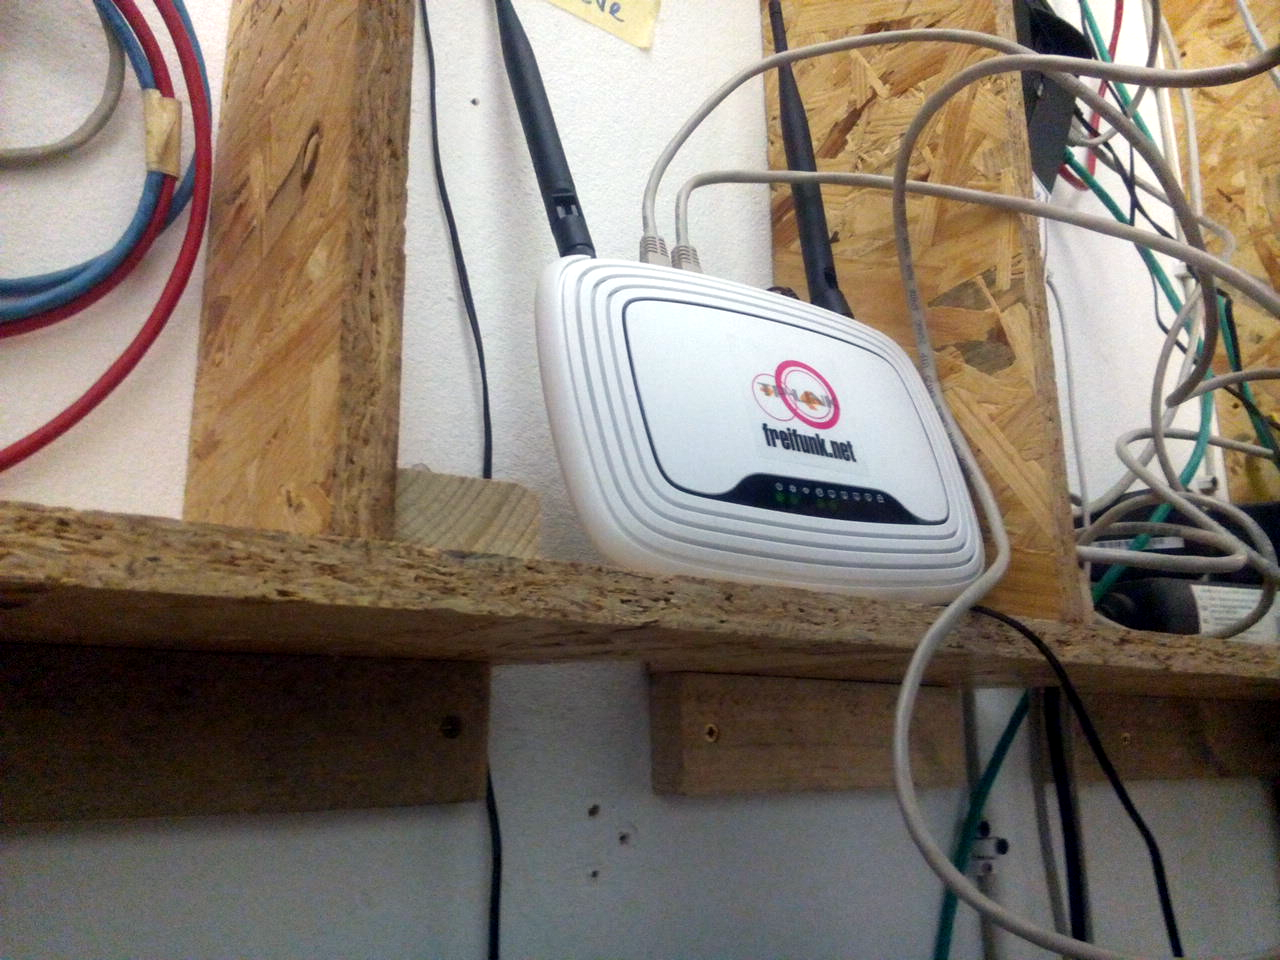
\includegraphics[width=0.7\textwidth]{irl_router}
\vfill
\end{frame}


\end{document}
